Антенна --- устройство, преобразующее энергию высокочастотного колебания от передатчика в электромагнитную волну, способную распространяться в пространстве. Или в случае приёма --- производит обратное преобразование (электромагнитную волну в ВЧ колебания)~\cite{habr:antenna}.

Простейшая антенна --- симметричный вибратор: два токопроводящих отрезка, каждый из которых равен 1/4 длины волны (рисунок~\ref{fig:symvibr}). Широко применяется для приема телевизионных передач, как самостоятельно, так и в составе комбинированных антенн. Так, к примеру, если диапазон метровых волн телепередач проходит через отметку 200 МГц, то длина волны будет равна 1,5 м. Каждый отрезок симметричного вибратора будет равен 0,375 метра.

\begin{figure}[ht]
    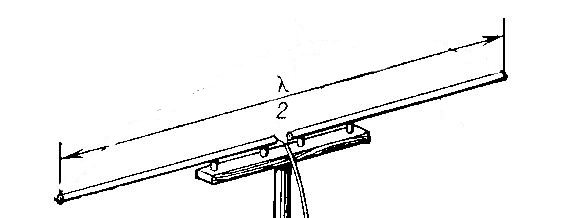
\includegraphics[width=.6\linewidth]{Figures/symvibr.jpg}
    \caption{Симметричный вибратор}
    \label{fig:symvibr}
\end{figure}

Несимметричный вибратор (штырьевая антенна) --- <<половина>> симметричного вибратора, установленного вертикально (рисунок~\ref{fig:asymvibr}). В качестве длины вибратора, применяют 1, 1/2 или 1/4 длины волны. Коэффициент направленного действия у несимметричного вибратора в два раза больше, чем у симметричного, за счет того, что вся мощность излучается в более узком направлении.

\begin{figure}[ht]
    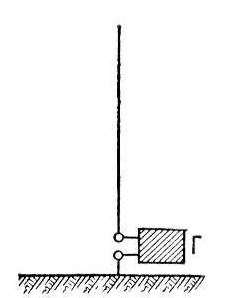
\includegraphics[width=.2\linewidth]{Figures/asymvibr.jpg}
    \caption{Несимметричный вибратор}
    \label{fig:asymvibr}
\end{figure}

При использовании приёмопередатчиков, работающих на частоте 433 МГц, длина волны $\lambda = 692$ мм. Соответственно, длина штырьевой антенны будет равна 69.2, 34.6 или 17.3 см.

Также существуют другие, более сложные типы антенн.

Поляризация --- это направленность вектора электрической составляющей электромагнитной волны в пространстве. Различают: вертикальную, горизонтальную и круговую поляризацию (рисунок~\ref{fig:polarization}).

\begin{figure}[ht]
    \subfloat[]{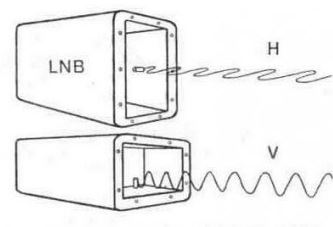
\includegraphics[width=.5\linewidth]{Figures/vgpolar.jpg}}
    \subfloat[]{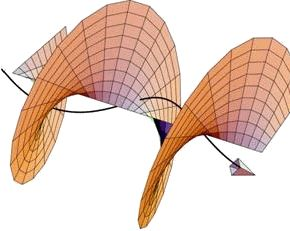
\includegraphics[width=.5\linewidth]{Figures/circlepolar.jpg}}
    \caption{Поляризация (а) горизонтальная и вертикальная; (б) круговая}
    \label{fig:polarization}
\end{figure}

Поляризация зависит от типа антенны и её расположения. К примеру, вертикально расположенный несимметричный вибратор, дает вертикальную поляризацию, а горизонтально расположенный --- горизонтальную.

Антенны горизонтальной поляризации дают больший эффект, т. к. природные и индустриальные помехи, имеют в основном вертикальную поляризацию. Горизонтально поляризованные волны, отражаются от препятствий менее интенсивно, чем вертикально. При распространении вертикально поляризованных волн, земная поверхность поглощает на 25\% меньше их энергии.
